\chapter{Analyse en ontwerp}\label{sec:anaEnOntwerp}
\section{Inleiding}
Uit de probleemstelling werd al snel duidelijk dat het probleem omtrent het installeren en updaten van programma's complexer is dan op het eerste zicht lijkt.
Bestaande systemen bieden geen geheel oplossing op de verscheidene problemen van Televic.
In dit hoofdstuk zal het probleem verder geanalyseerd worden.
Aan de hand van deze bevindingen gaat een architectuur ontworpen of geselecteerd worden die aan de basis gaat liggen voor de demo.
Het doel van de demo is het weergeven van de volledige installatieproces startende van het toevoegen van een testtoren aan het systeem tot en met het uitbrengen en installeren van een nieuwe versie van het Python testraamwerk.
Deze demo geeft Televic ook een goede basis waarop later kan worden verder gewerkt.

\section{Analyse}
Het probleem van Televic was het volgende:
Televic fabriceert producten die moeten voldoen aan strenge veiligheidsnormen.
Om hun producten hierop te kunnen testen heeft Televic een Python testraamwerk ontworpen waarmee het mogelijk wordt om de producten aan verschillende testscenario's te onderwerpen.
Dit testraamwerk maakt gebruik van een grote set aan drivers en bibliotheken om een correcte werking te garanderen.
Een direct gevolg hiervan is dat het installatieproces op een nieuwe testtoren veel tijd in beslag neemt en foutgevoelig is.
Het is belangrijk om rekening te houden met deze fouten en een rampenplan te voorzien.
Hiernaast groeit het aantal gebruikers van het testraamwerk continu samen met het aantal drivers, bibliotheken en programma's die verspreid moeten worden.
Verder dient elk nieuw toestel op het raamwerk ondersteund te worden waardoor er jaarlijks ettelijke releases van het raamwerk verspreid moeten worden.
Er moet dus een antwoord gegeven worden op de volgende vragen:
\begin{itemize}
\item Wat moet verzonden worden naar de gebruikers?
\item Hoe raakt de software van de producent bij de gebruikers?
\end{itemize}
Het doel is om een systeem te ontwikkelen dat Televic kan bijstaan bij het installatieproces en verspreidingsproces maar ook om een systeem te ontwikkelen dat kan blijven gebruikt worden in de toekomst.
Schaalbaarheid en flexibiliteit zijn hierbij zeer belangrijk.

%Packager
De probleemanalyse onthulde dus dat het probleem onder te verdelen is in verschillende deelproblemen (Wat wordt verzonden en hoe wordt dit aangepakt).
Het testraamwerk bestaat uit verschillende componenten, hieronder vallen de drivers en bibliotheken.
Elke component heeft een aparte installatiewijze en sommige componenten moeten voor andere geïnstalleerd worden.
Zo zal Python één van de eerste componenten zijn die geïnstalleerd moet worden.
Hiernaast moeten verscheidene componenten geconfigureerd tijdens het installatieproces aan de hand van een configuratiebestand.
Dit configuratiebestand is afhankelijk van testtoren waarop het testraamwerk op geïnstalleerd word.
Door gebruik te maken van additionele software worden verschillen in implementaties, door bijvoorbeeld verschillende programmeertalen, opgevangen.
Een deel van de applicatie zal dus bestaan uit deze additionele software die instaat voor het inpakken van de componenten: de \emph{packager}.
Hiervoor kan beroep gedaan worden op verscheidene technologieën, structuren en architecturen die besproken werden in Sectie~\ref{sec:technologieen}.
Door gebruik te maken van één van deze technologieën is geweten wat er wordt verzonden.

%Server
Naast de wat moet er ook geweten zijn hoe de software bij de gebruikers moet geraken.
Door dit proces te automatiseren, is het mogelijk om waardevolle informatie te verzamelen.
Met deze informatie kunnen rapporten gegeneerd worden over het deployment proces.
In Secties~\ref{sec:deployment} - \ref{sec:caseStudies} werden verschillende problemen maar ook oplossingen besproken die aan de basis liggen voor het ontwerp van dit onderdeel van de applicatie. 
In het vervolg van de thesis zal dit onderdeel (dat zal instaan voor het verspreiden van het testraamwerk maar ook voor de communicatie tussen de producten van het testraamwerk en de gebruikers) vermeld worden als de \emph{deployment server}.

%Environment
In Sectie~\vref{sec:softwareLevenscyclus} werd besproken welke problemen kunnen optreden tijdens het installatieproces.
Deze problemen moeten opgevangen worden om een schaalbare oplossing te bedenken voor Televic.
Om dit op te vangen, kan er gebruik gemaakt worden van één (of meerdere) strategieën die besproken werd in Sectie~\vref{sec:rollback}.
Dit onderdeel van de applicatie vooral aanwezig aan de client-side aangezien dat de plaats is waar het testraamwerk aanwezig zal zijn.
In de loop van de thesis zal naar dit onderdeel verwezen worden als de \emph{deployment environment}.

%%% TODO Schrijven over databank

Na de probleemanalyse is het nu duidelijk dat het werk op te delen valt in vier grote componenten.
Deze vier onderdelen zullen de basis vormen voor de architectuur en zullen gebruikt worden als leidraad.
Het eerste onderdeel zal bestaan uit de packager met als doel het inpakken van de nodige drivers, bibliotheken, \ldots .
Naast de packager bestaat de deployment server die instaat is om de installers die de packager aflevert te verspreiden naar de verschillende gebruikers.
Aan de client-side zal de deployment environment aanwezig zijn waardoor installatie-complicaties verminderd worden door de installatie te isoleren.
Mocht een rollback nodig zijn, dan kan deze op een eenvoudige manier gebeuren.
In Figuur~\vref{fig:overzichtsDiagram} wordt de algemene structuur van de applicatie weergegeven.
Met behulp van deze basis is het mogelijk om een demo te produceren voor de finale verdediging.

\begin{figure}[!hbt]
\centering
  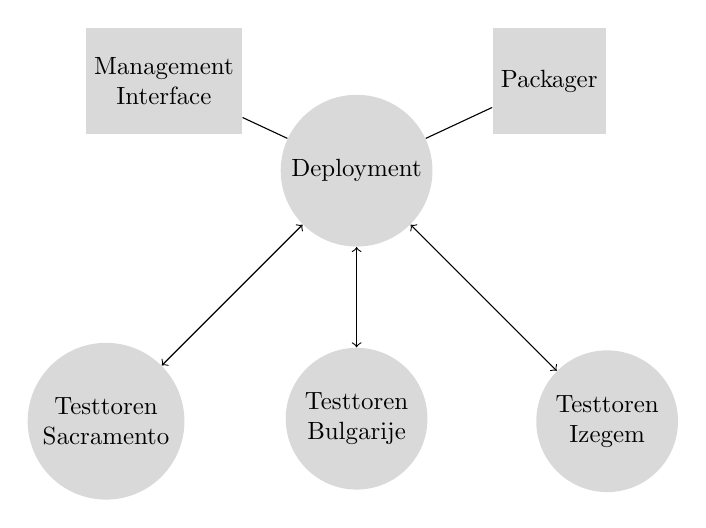
\begin{tikzpicture}[scale=.9, transform shape]
\tikzstyle{every node} = [circle, minimum size = 2cm, fill=gray!30]
\node (a) at (0, 0) {Deployment};
\node[shape = rectangle,minimum size = 1.5cm] (packager) at +(25: 3) {Packager};
\node[shape = rectangle,minimum size = 1.5cm, align=center] (logger) at +(155: 3) {Management\\ Interface};
\node[align=center] (b) at +(225: 5) {Testtoren\\ Sacramento};
\node[align=center] (c) at +(270: 3.5) {Testtoren\\ Bulgarije};
\node[align=center] (d) at +(315: 5) {Testtoren\\ Izegem};
\foreach \from/\to in {a/b, a/c, a/d}
\draw [<->] (\from) -- (\to);
\draw [-] (a) -- (packager);
\draw [-] (a) -- (logger);
\end{tikzpicture}
  \caption{Overzichtsdiagram van de algemene structuur}
  \label{fig:overzichtsDiagram}
\end{figure}

\section{Architectuur}
Huidige architecturen en technologieën voldoen niet aan de verwachtingen en bieden geen sluitende oplossing voor alle problemen van Televic.
Meeste technologieën bieden een deeloplossing aan.
Zo biedt de LJSFi architectuur van ATLAS een mooie oplossing aan voor het verspreiden van verschillende software pakketten naar een groot aantal computers maar bij deze architectuur moet gebruik gemaakt worden van de Grid middleware.
De Redhat package manager biedt een volledig beschikbare infrastructuur aan maar afhankelijkheden tussen pakketten zijn dan weer minder goed gedefinieerd.
De drie lagen architectuur is een goede architectuur voor het verspreiden van de software maar biedt geen mogelijkheden aan voor de installatie van software pakketten.
Om toch een oplossing te bieden voor de problemen wordt zelf een architectuur ontworpen die bestaat uit een combinatie van besproken technologieën en architecturen.

Zoals in de analyse al werd aangehaald, zal de architectuur bestaan uit de volgende componenten: 
\begin{itemize}
\item De deployment server
\item De packager
\item De database
\item De deployment client
\end{itemize}
Figuur~\vref{fig:architectuur} geeft de volledig ontworpen architectuur weer.

\begin{sidewaysfigure}
\includegraphics[width=\textwidth,height=\textheight,keepaspectratio]{afbeelding/architectuur.png}
\centering
\caption{Architectuur van het prototype}
\label{fig:architectuur}
\end{sidewaysfigure}

De basis van de architectuur is overgenomen van de software dock architectuur uit Sectie~\ref{sec:softwareDock}.
Door gebruik te maken deze architectuur is het mogelijk om de deployment server samen met de packager te combineren tot een release dock en de deployment client te implementeren als een field dock. 
Het gebruik van software dock zorgt voor een schaalbare architectuur waarbij het aantal gebruikers en producenten mag toenemen.
Zowel het release dock als het field dock moet niet bijhouden welke docks aanwezig zijn in het netwerk aangezien dit de taak is van de broker.
Verder zorgen de agenten voor een verhoogde flexibiliteit in alle stappen van de deployment levenscyclus.
Technologieën zoals ElectricFlow en ATLAS gebruiken ook agenten voor het installeren van software.
Bij deze technologieën zijn de agenten afgestemd op de software die moet geïnstalleerd worden en niet op een stap uit de deployment levenscyclus.

Om de functionaliteiten van de packager te implementeren wordt een systeem ontworpen dat gebaseerd is op het Qt installer framework.
Andere software packaging oplossingen (zoals NSIS en WiX Toolset) bieden ook een oplossing voor het combineren van software pakketten.
Er wordt toch voor het Qt installer framework gekozen omdat software pakketten beter van elkaar gescheiden worden.
Dit geeft een beter overzicht van wat aanwezig is in een installer en welke installatiescripts uit de meta folder invloed heeft op de data.
Door gebruik te maken van een gelijkaardige structuur wordt een packager ontworpen die kan omgaan met verschillende types van software pakketten.
Het Qt installer framework zelf volstaat niet aangezien het niet mogelijk is om op één besturingssysteem een installer te creëren die werkt op zowel Linux als Windows.
Aangezien de packager zelf ontworpen wordt, is het mogelijk om eender welke programmeertaal te kiezen.
Er wordt dus best een taal gekozen die volledig besturingssysteem-onafhankelijk is.
Door deze packager te combineren met de software dock architectuur is het mogelijk om naast het personaliseren van iedere stap in het deployment proces ook de behandeling van ieder software pakket apart te personaliseren.
De packager wordt opgenomen in de code van het release dock en wordt door gebruikt om installers te produceren.

Een laatste element uit de architectuur is de deployment omgeving die zal bestaan uit het field dock van de software dock architectuur.
Het doel van de deployment omgeving is het creëren van een veilige omgeving waarin de installer van het release dock in geïnstalleerd en geüpdatet kan worden.
Zoals reeds werd aangegeven is het installatieproces en updateproces foutgevoelig en moet hiervoor een oplossing gevonden worden.
Dit wordt dan ook opgelost door Docker containers te gebruiken.
Er wordt niet gekozen voor één van de rollback strategieën aangezien deze ofwel een beperking opleggen (zoals het gebruik moeten maken van het transactieprogrammeermodel) of veroorzaken extra overhead (zoals bij het gebruiken van checkpoints).
Virtuele machines kunnen eventueel ook gebruikt worden als oplossing.
Bij het optreden van een fout kan de VM verwijdert worden zodanig dat er geen software achterblijft die later voor problemen kan zorgen.
Het nadeel van virtuele machines is dat acties die uitgevoerd worden op VMs lang duren.
Docker containers hebben dit probleem niet.
Er wordt een veilige omgeving gecreëerd die snel opgestart en afgebroken kan worden.

Na het ontwerpen van de algemene architectuur wordt een klassendiagram en deployment diagram ontworpen die gebruikt worden voor de implementatie.
Figuur~\vref{fig:classDiagram} geeft het klassendiagram weer en Figuur~\vref{fig:deploymentDiagram} het deployment diagram.
Uit het deployment diagram wordt het snel duidelijk dat de server de meeste componenten bevat.
In wat volgt, wordt dieper ingegaan op de vier componenten waaruit de architectuur bestaat aan de hand van het klassendiagram en het deployment diagram.

\begin{figure}[!ht]
\centering
\makebox[0pt]{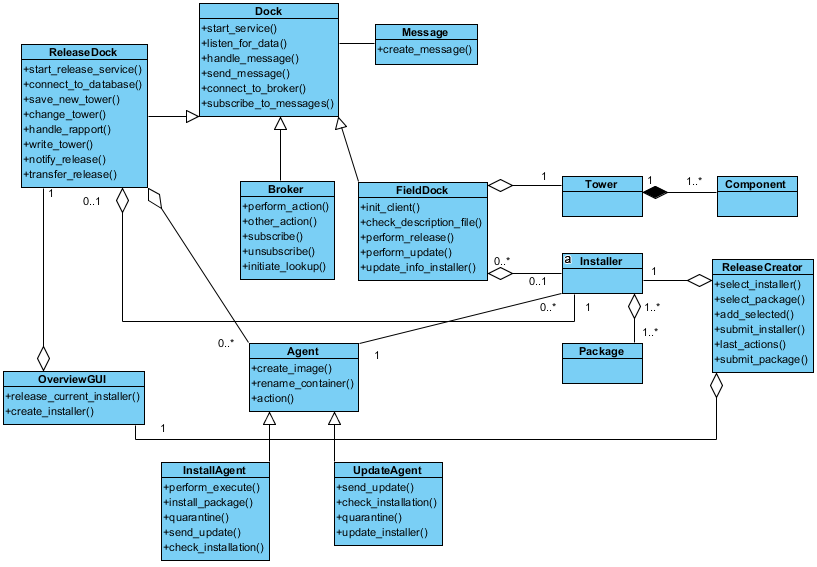
\includegraphics[width=\textwidth]{afbeelding/classDiagram.png}}
\caption{Klassendiagram van de applicatie}
\label{fig:classDiagram}
\makebox[0pt]{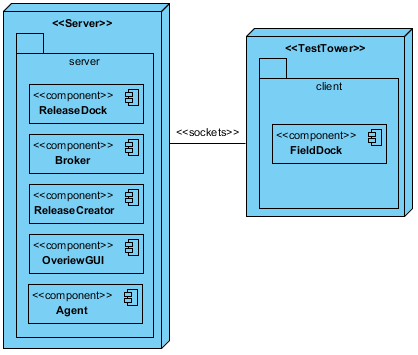
\includegraphics[scale=1]{afbeelding/deploymentDiagram.png}}
\caption{Deployment diagram van de applicatie}
\label{fig:deploymentDiagram}
\end{figure}
\clearpage

\subsection{Deployment server}
Het centrale systeem in de architectuur is de deployment server.
Zoals reeds uitgelegd zal dit onderdeel instaan voor het verspreiden van de verschillende installers en functioneren als een verzamelcenter voor alle informatie.
De software dock architectuur bestaat uit 4 grote componenten, namelijk het release dock, field dock, event service en de agenten (zie figuur~\ref{fig:architectuur}).
Alle componenten behalve het field dock zijn aanwezig aan de serverzijde.

\subsubsection{Release Dock}
Uit het klassendiagram in Figuur~\ref{fig:classDiagram} wordt al snel duidelijk dat de ReleaseDock klasse geassocieerd kan worden met de OverviewGUI klasse en ReleaseCreator klasse.
Dit wordt is ook duidelijk zichtbaar in het deployment diagram waarin weergegeven wordt dat deze drie aanwezig zijn op één server.
De belangrijkste functionaliteiten van het release dock bestaat uit het wegschrijven van informatie naar de databank en het afhandelen van de verschillende release aanvragen.
De weg te schrijven informatie bestaat vooral uit gegenereerde rapporten van verscheidene testen maar ook nieuwe gebruikers die moeten toegevoegd worden aan de databank.

De OverviewGUI klasse wordt ontworpen als managersinterface.
De grafische user interface die hiervoor ontworpen werd, is terug te vinden in Figuur~\vref{fig:overviewGUI}.
Het doel is om de informatie die aanwezig is in de database weer te geven.
Op deze wijze is het mogelijk om een overzicht te geven van alle clients die verbonden zijn met het systeem maar ook welke software zij gebruiken.
Door dit overzicht krijgt Televic een algemeen beeld van hoe het verspreiden van hun software verloopt.

\begin{figure}[!ht]
\centering
\makebox[0pt]{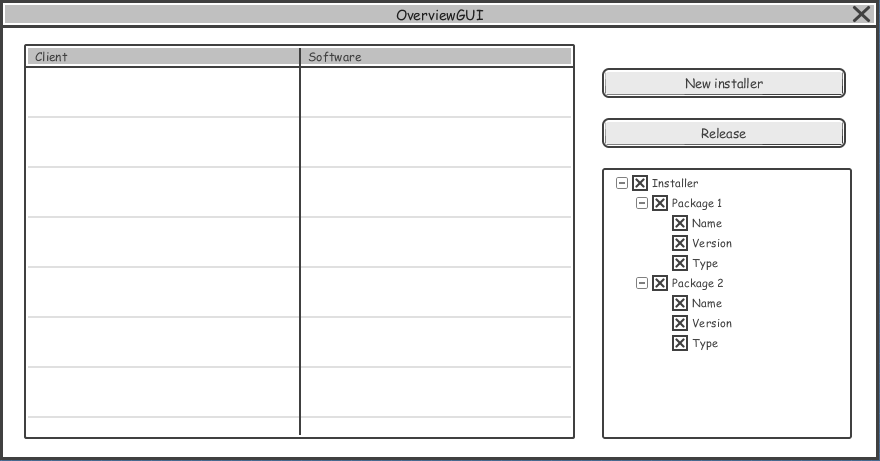
\includegraphics[scale=0.5]{afbeelding/overViewGUI.png}}
\caption{Ontwerp van de managersinterface}
\label{fig:overviewGUI}
\end{figure}

\begin{figure}[!ht]
\centering
\makebox[0pt]{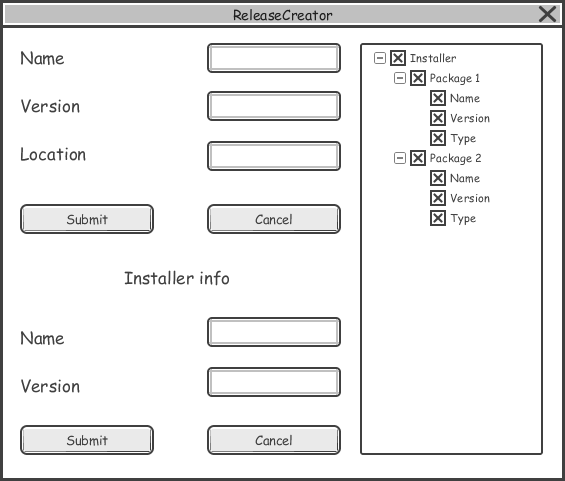
\includegraphics[scale=0.5]{afbeelding/releaseCreator.png}}
\caption{Ontwerp van de release creatie interface}
\label{fig:releaseCreator}
\end{figure}

Het release dock is indirect verbonden met de ReleaseCreator.
Dit is de grafische user interface die instaat voor het creëren van een nieuwe release indien dit nodig is.
Figuur~\ref{fig:releaseCreator} geeft het ontwerp van de grafische user interface weer.
Zoals reeds werd toegelicht, zal een installer bestaan uit verschillende software pakketten.
Hoe een installer exact wordt opgebouwd en welke bestanden worden aangemaakt, wordt verderop besproken.
Na het creëren van de installer wordt deze doorgegeven aan de ReleaseDock.
Vanaf dat moment is het mogelijk om vanuit de OverviewGUI de installer op te geven voor release.

\subsubsection{Event Service}
Naast de verschillende docks beschrijft de software dock architectuur een Event Service.
Deze staat in voor het afhandelen van de communicatie tussen de verschillende docks.
Om dit te implementeren, wordt er beroep gedaan op Sectie~\vref{sec:event}.
Er worden evenwel enkele kleine aanpassingen gemaakt aan het formaat van de publish/subscribe eventen.
Er wordt een eigen formaat ontworpen zodanig dat alle nodige elementen zeker in een bericht vervat zit.
Hiernaast wordt de Broker klasse zo ontworpen dat er slechts één broker aanwezig kan zijn.
Dit zorgt voor een vereenvoudiging van de implementatie aangezien geen protocollen voorzien moeten worden om tussen verschillende brokers te kunnen communiceren.
Het is wel belangrijk om hierbij te vermelden dat dit een impact heeft op de schaalbaarheid van de applicatie.
Van zodra een te groot aantal docks aanwezig is, zal de broker een bottleneck vormen voor de applicatie.
Dit wordt in een verder hoofdstuk nog besproken.

Bij de broker worden verschillende lijsten bijgehouden voor ieder type van bericht dat mogelijk is.
Bij het toekomen van een subscribe/unsubscribe bericht, zal de broker de nodige lijsten aanpassen zodat de zender van het bericht wordt toegevoegd of verwijderd.
Berichten in het netwerk zullen bestaan uit een set van attributen en waarden in een JSON formaat.
Het uiterlijk van zo'n bericht is gelijkaardig als het uiterlijk van een bericht in Figuur~\vref{fig:pubsubNot}.
In Listing~\vref{list:bericht} wordt een voorbeeld van een bericht weergegeven.
Ieder bericht heeft dezelfde set aan attributen die elk een eigen functie hebben:
\begin{itemize}
\item \emph{Timestamp}: ieder bericht zal op het moment van de creatie een timestamp krijgen.
De timestamp wordt uitgedrukt in seconden sinds epoch.
Op deze wijze wordt eenzelfde referentie punt gebruikt en is het mogelijk om de creatie van berichten in de tijd te ordenen.
\item \emph{Type}: ieder bericht hoort toe aan een bepaald type.
De verschillende types van berichten zijn: subscribe, unsubscribe, new, change, rapport, update, release.
Afhankelijk van het type bericht dat toekomt, bij zowel de broker als een dock, zal een andere actie ondernomen worden.
De eerste twee types zijn uitsluitend bedoeld voor de broker.
De volgende drie voor een release dock en de laatste twee voor de field docks.
\item \emph{ID}: naast een timestamp wordt aan ieder bericht een id meegegeven. 
Dit attribuut wordt meegegeven zodanig dat de field docks kunnen achterhalen of zij achterlopen op berichten.
\item \emph{Data}: Dit is het meest flexibele attribuut. 
Hier wordt de data meegegeven die hoort bij het bericht.
Als het type van een bericht ``subscribe'' is, dan zit in het data veld een lijst met alle types waarvoor de gebruiker zich voor wilt inschrijven.
\item \emph{Sender}: Het laatste attribuut dat wordt meegegeven is de zender van het bericht.
De broker moet bij een subscribe bericht kunnen achterhalen wie de zender is.
Op die manier weet de broker wie moet worden toegevoegd aan de nodige lijsten.
\end{itemize}

\begin{minipage}{\linewidth}
\begin{center}
\begin{lstlisting}[caption={Formaat voor een bericht},label={list:bericht}, xleftmargin=.3\textwidth]
{
 'timestamp': 1491982212.555,
 'type': 'subscribe',
 'id': 0,
 'data': {
   'type': [
     'new',
     'change',
     'rapport'
   ]
 },
 'sender': 'localhost'
}
\end{lstlisting}
\end{center}
\end{minipage}

\subsubsection{Agenten}
%%schrijven over hoe de agenten werken en hoe ze gaan werken volgens de handelingen van ORYA
Een laatste element die aangemaakt wordt aan de serverzijde zijn de agenten.
Deze staan in voor het uitvoeren van allerlei deployment gerelateerde handelingen.
Iedere agent is gekoppeld aan één stap uit de software levenscyclus die besproken werd in Sectie~\ref{sec:softwareLevenscyclus}.
Hiernaast zal aan iedere installer afkomstig van het release dock een subset van alle agenten toegevoegd en verscheept worden naar het field dock.
Op deze manier is het mogelijk om iedere stap in de levenscyclus van de installer te personaliseren.
Ieder agent zal een bepaalde set van handelingen uitvoeren die overeenkomt met een deployment proces die besproken werd in de ORYA case studie in Sectie~\ref{sec:ORYA}.
Net zoals bij ORYA wordt ieder deployment proces beschreven aan de hand van andere deployment processen en basis activiteiten.
Zo zal tijdens de creatie van een installer een agent voorzien worden die instaat voor het installatieproces.
De agent wordt samen met de installer verscheept naar het field dock waarna de agent op het gepaste moment in actie schiet.
De agent begint met het hernoemen van de oude Docker container met daarin de vorige versie van een installer.
Hierna wordt een nieuwe container aangemaakt waarin de nieuwe installer wordt losgelaten.
Vervolgens zal de agent de installatie aanvangen en zullen de scripts horende bij de pakketten uitgevoerd worden in de container.
Zoals reeds werd aangegeven, zijn de handelingen van een agent gebaseerd op het model van ORYA.
Zo wordt het creëren van een nieuwe container in de installatie agent gezien als zo'n basis activiteit.
In Bijlage~\ref{sec:flowcharts} zijn verschillende activiteitendiagrammen terug te vinden die horen bij enkele types van agenten.
Door agenten te gebruiken, een strategie die ook gezien werd in de Atlas case studie in Sectie~\ref{sec:ATLAS}, wordt het mogelijk om alle stappen in de software levenscyclus uniek te behandelen.
Hiernaast kan bij iedere installer een andere set van agenten geassocieerd worden waardoor iedere installer verder gepersonaliseerd kan worden.

\subsubsection{Initialisatie}\label{sec:initServer}
Het deployment diagram in Figuur~\vref{fig:deploymentDiagram} geeft weer dat aan de serverzijde verschillende componenten aanwezig zijn die samenwerken.
Hierbij is het belangrijk om een goede opstartsequentie te voorzien.
Figuur~\vref{fig:seqStartServer} geeft weer hoe de nodige componenten opgestart worden.

\begin{figure}[!ht]
\centering
\makebox[0pt]{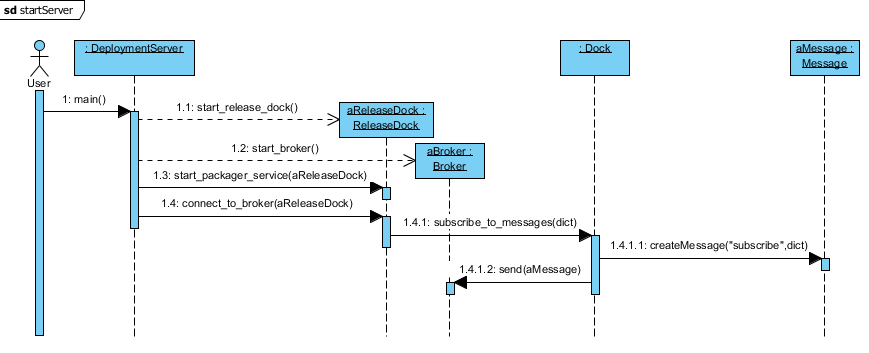
\includegraphics[scale=0.6]{afbeelding/seqStartServer.png}}
\caption{Sequentie diagram voor het opstarten van een server}
\label{fig:seqStartServer}
\end{figure}

Als eerste wordt een ReleaseDock object aangemaakt, gevolgd door een Broker object.
Uit het klassendiagram in Figuur~\ref{fig:classDiagram} blijkt dat beide objecten van hetzelfde object overerven.
Dit werd zo ontworpen aangezien beide objecten dezelfde functionaliteiten moeten implementeren (namelijk het verzenden van berichten, het luisteren voor nieuwe data en het afhandelen van binnenkomende berichten).
Vervolgens zal het release dock zich gaan inschrijven voor berichten met als type new, change, en rapport.
Nadat de nodige services zijn opgestart is het mogelijk om de overviewGUI op te starten.

\subsection{Packager}
De architectuur van de packager wordt gebaseerd op de architectuur van het Qt installer framework.
Er wordt een installer geproduceerd die bestaat uit verschillende pakketten die elk instaan voor het installeren van een software component.
Voor iedere installer wordt een aparte folder structuur aangemaakt die zichtbaar is in Figuur~\vref{fig:installerStructuur}.

\begin{figure}[!ht]
\centering
\makebox[0pt]{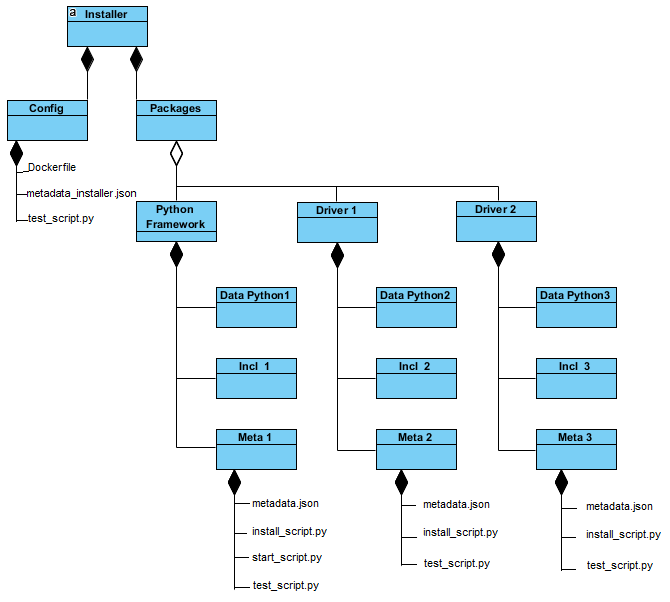
\includegraphics[scale=0.7]{afbeelding/folderStructure.png}}
\caption{Structuur van een installer bestaande uit drie pakketten}
\label{fig:installerStructuur}
\end{figure}

Door zelf een packager te produceren, is het mogelijk om iedere stap in het deployment proces te personaliseren.
Op deze manier kan na het installeren van een pakket een zo optimaal mogelijke afhandeling plaats vinden.
Zo kunnen testen op ieder moment in het installatieproces toegevoegd worden, een handeling die met het Qt installer framework ook mogelijk is maar dit is moeilijker te realiseren.
Hiernaast kan ervoor gezorgd worden dat de software pakketten beter overweg kunnen met Docker.
Zo is er een vlottere integratie van Docker.

In de config folder van de installer worden alle globale scripts en beschrijvingsbestanden bijgehouden.
Verder bevat de installer subtrees voor ieder pakket.
Een pakket bestaat vervolgens uit een data, include en meta folder.
De data folder wordt gebruikt om de effectieve driver/bibliotheek in op te slaan.
Hiernaast is een include folder aanwezig waarin verschillende afzonderlijke scripts toegevoegd kunnen worden.
Op deze manier kunnen willekeurige scripts (bijvoorbeeld een script die de firewall instellingen aanpast) rap toegevoegd worden aan een pakket.
Als laatste bevat de meta folder alle meta-data horende het pakket.

Tijdens het creëren van de installer moet één van de pakketten aangeduid worden als een framework pakket.
Bij het toevoegen van de verschillende bestanden zal dit pakket een start\_script meekrijgen.
Dit is het script dat wordt uitgevoerd iedere keer als het framework wordt opgestart.
Hierna worden alle pakketten overlopen.
Als het pakket nieuw is, worden de nodige folders en bestanden aangemaakt anders worden de oude bestanden uit de meta folder gekopieerd.
Nadat de folder structuur aangemaakt is, is het mogelijk om de verschillende scripts aan te passen.
Net als bij het QT Installer Framework is het de bedoeling om te scripts te personaliseren naargelang het pakket.
Op deze wijze heeft ieder pakket een uniek installatie en test proces.
De installer is hierna klaar om gereleased te worden.

Vanuit de Overview is het mogelijk om een installer te releasen.
Figuur~\vref{fig:releaseSeq} geeft het sequentie diagram weer dat gevolgd wordt om de installer van het release dock naar het field dock te brengen.
Het release dock maakt een Message object aan, geeft de installer informatie mee en zet het type van het bericht op release.
Vervolgens wordt deze doorgestuurd naar de broker.
Deze zal op zijn beurt het bericht inpakken als een notificatie bericht en het nieuwe bericht doorsturen naar de docks die voor release gesubscribed zijn.
Met de informatie uit het bericht is het field dock in staat om een Installer object te maken.
Het field dock achterhaalt wie de zender van het bericht en contacteert dan direct de zender\footnote{Dit is het enige moment dat directe communicatie tussen de field en release docks mogelijk is}.
Nadat een connectie tussen de twee werd opgestart, wordt de gezipte installer samen met de nodige agenten verzonden naar het field.
De lijst van agenten wordt overlopen en het install agent object zal zijn functie uitvoeren.

\begin{sidewaysfigure}
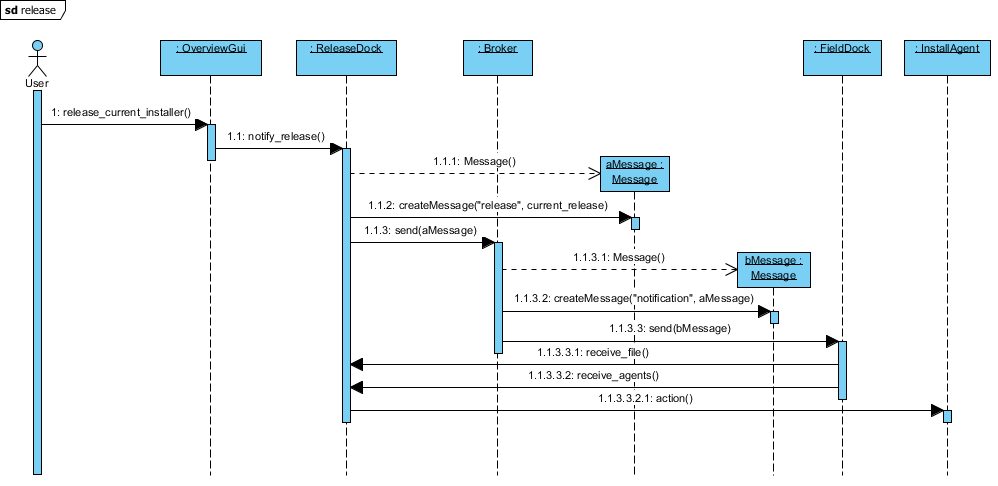
\includegraphics[width=\textwidth,height=\textheight,keepaspectratio]{afbeelding/seqRelease.png}
\centering
\caption{Sequentie diagram voor het releasen van een installer}
\label{fig:releaseSeq}
\end{sidewaysfigure}

\subsection{Databank ontwerp}\label{sec:databank}
Eén van de problemen is de continue toename aan pakketten waar het framework gebruikt van maakt en het aantal gebruikers die het framework gebruiken.
Om dit probleem aan te pakken wordt een databank ontworpen voor het opslaan van alle cruciale data over zowel het installatieproces en als de gebruikers.
In overleg met Televic werd ervoor gekozen om MySQL te gebruiken als databasesysteem.
Het ontwerp van de databank is terug te vinden in Figuur~\ref{fig:databank}.

\begin{figure}[!ht]
\centering
\makebox[0pt]{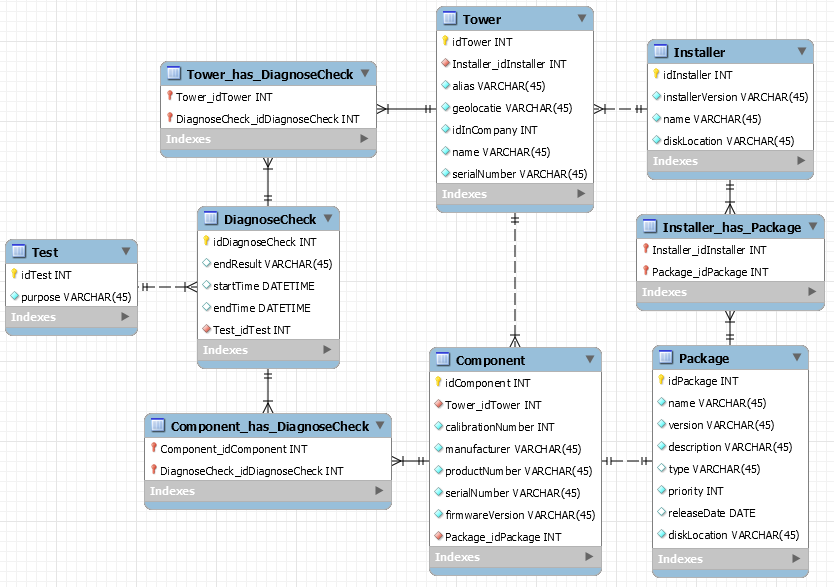
\includegraphics[scale=0.7]{afbeelding/databankOntwerp.png}}
\caption{Ontwerp van de databank}
\label{fig:databank}
\end{figure}

De tabellen tower en hardware\_component dienen om iedere gebruiker, typisch een testtoren of een laptop, te beschrijven.
Iedere toren heeft een ID, naam en serienummer.
De combinatie van deze drie waarden is uniek binnen het bedrijf en de combinatie kan gebruikt worden als identificatie binnen het systeem maar deze combinatie draagt geen betekenis voor een gebruiker.
Om dit op te vangen wordt aan iedere toren een alias gekoppeld waardoor de identificatie voor mensen vlotter kan verlopen.
Elke toren bestaat typisch uit verschillende hardwarecomponenten, zoals voedingen of netwerkkaarten, die nodig zijn om testen uit te voeren.
Iedere component is gemaakt door een bepaalde fabrikant en krijgt van de fabrikant een serienummer.
Vanuit het bedrijf wordt losstaand hiervan een nummer toegekend aan iedere component die gebruikt wordt om de calibratie instellingen te achterhalen.
Iedere hardwarecomponent gebruikt firmware om correct te functioneren.
Naast alle bovengenoemde informatie wordt ook de versie van de firmware opgeslagen.
Door het opslaan van al deze informatie wordt het mogelijk om:
\begin{enumerate}
\item Torens van elkaar te onderscheiden
\item Hardware componenten te koppelen aan torens
\item Firmware versies te koppelen aan hardware componenten
\end{enumerate}

Naast informatie over de gebruikers wordt ook informatie over de verschillende installers en pakketten bijgehouden.
Een installer bestaat uit een combinatie van verschillende software pakketten.
Bij deze pakketten moet één pakket aanwezig zijn dat het Python testraamwerk bevat.
Hiernaast zijn verschillende andere pakketten aanwezig voor drivers.
In Figuur~\vref{fig:installerStructuur} is een voorbeeld zichtbaar van een installer die bestaat uit drie verschillende pakketten.
Eén pakket wordt gebruikt door het testraamwerk en de twee anderen voor drivers die nodig zijn om het testraamwerk correct te laten functioneren.
Iedere toren wordt gekoppeld aan één installer en zo aan één testraamwerk.
Hiernaast is het mogelijk om pakketten te koppelen aan hardware componenten.
Zo kan een driver voor een voeding gekoppeld worden aan de entry van de voeding die aanwezig is in de hardware\_component tabel.
Op deze wijze worden de hardware-software afhankelijkheden bijgehouden.
Van ieder pakket wordt bijgehouden welk type pakket het is (een executabel, zip bestand, \ldots), de prioriteit voor de installatievolgorde, een korte beschrijving en de release datum.
Naast al deze informatie wordt er ook bijgehouden welke pakketten afhankelijk zijn van elkaar.
Een voorbeeld is hiervan is een testraamwerkpakket en een pakket waarmee Python geïnstalleerd wordt.
Het testraamwerk is afhankelijk van Python om correct te functioneren.
Zo worden de verschillende software-software afhankelijkheden bijgehouden.
Voordat een installer gemaakt wordt, die een testraamwerkpakket bevat, kan gecontroleerd worden dat ook het Python-installatiepakket aanwezig is.

Verder zijn er enkele tabellen aanwezig voor het ondersteunen van testen.
Tijdens en na het installatieproces moet het mogelijk zijn om testen uit te voeren.
Dankzij deze testen is het duidelijk of een bepaald pakket correct functioneert en op het einde van het installatieproces kan gecontroleerd worden of het volledige testraamwerk in zijn geheel functioneert.
Doordat er een link wordt bijgehouden tussen een hardware component en een pakket, is het mogelijk om hieruit waardevolle informatie te halen.
Zo kan bijvoorbeeld een verband gelegd worden tussen een bepaalde versie van een driver en de firmware die aanwezig is in een hardware component.
Deze informatie kan gebruikt worden om problemen in testtorens te vermijden.

\subsection{Deployment environment}
De deployment environment komt overeen met de field dock in de software dock architectuur.
In de omgeving gaat de installer, afkomstig van de packager, uitgevoerd worden zodat de software geïnstalleerd wordt.
Aan dit proces zijn de volgende problemen verbonden die grondig besproken werden in Sectie~\ref{sec:softwareLevenscyclus}.

Het opstarten van een client gebeurd op een gelijkaardige manier als het opstarten van een server.
Figuur~\vref{fig:seqClient} bevat het sequentie diagram voor het opstarten van een client.
Hiervoor wordt eerst een FieldDock aangemaakt en deze zal zich vervolgens bij de broker inschrijven voor berichten van het type release en update.
Bij het eerst gebruik moet het systeem eerst beschreven worden zodanig dat deze beschrijving toegevoegd kan worden aan de database.
Het ontwerp van de grafische user interface is terug te vinden in Figuur~\vref{fig:startClient}.
Na het registeren van de client kan de gebruiker gebruik maken van de grafische user interface in Figuur~\vref{fig:overviewClient}.
Van hieruit is het mogelijk om nieuwe software die van het release dock te beoordelen en eventueel te installer.

\begin{figure}[!ht]
\centering
\makebox[0pt]{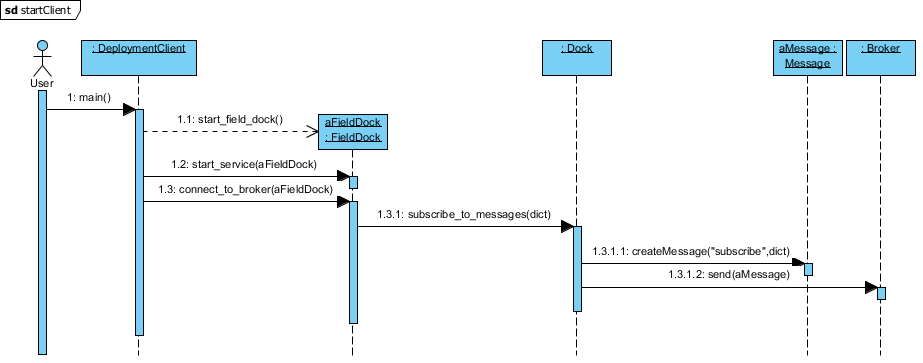
\includegraphics[scale=0.6]{afbeelding/seqStartClient.png}}
\caption{Sequentie diagram voor het opstarten van een client}
\label{fig:seqClient}
\end{figure}

Om de verschillende deploymentproblemen te vermijden en om ervoor te zorgen dat er geen uitgebreide rollback strategieën nodig zijn, wordt een geïsoleerde omgeving voorzien waarin de software geïnstalleerd wordt. 
Dit wordt gerealiseerd aan de hand van virtualisatietechnieken, meer bepaald aan de hand van Docker.
Docker wordt verkozen boven een gewone virtuele machine omdat het uitvoeren van handelingen (zoals opstarten, stoppen, \ldots) op een container minder resources en tijd vraagt in vergelijking met een virtuele machine.
Doordat een virtualisatietechniek wordt gebruikt, wordt het zeer eenvoudig om problemen tijdens de verschillende processen op te vangen.
In Figuur~\vref{fig:flow:rollback} is het duidelijk dat, door het gebruik van Docker, het rollback proces zeer eenvoudig is.
Hierbij is het belangrijk om te weten dat de container met de defecte code niet wordt verwijdert.
De defecte code wordt in ``quarantaine'' geplaatst.
Mochten logische fouten aanwezig zijn in een test kan dit leiden tot het afkeuren van de software terwijl de installatie wel correct verlopen is.
Door de container in quarantaine te plaatsen is het mogelijk om na het installatieproces de container te ondervragen en te achterhalen wat fout gelopen is.
Figuur~\vref{fig:fieldDock} geeft weer op welke manier de agenten met de containers gaan communiceren en geeft ook weer hoe Docker wordt geïntegreerd in het geheel.

\begin{figure}[!ht]
\centering
\makebox[0pt]{\includegraphics[width=\textwidth]{afbeelding/fieldDock.png}}
\caption{Structuur van een field dock}
\label{fig:fieldDock}

\makebox[0pt]{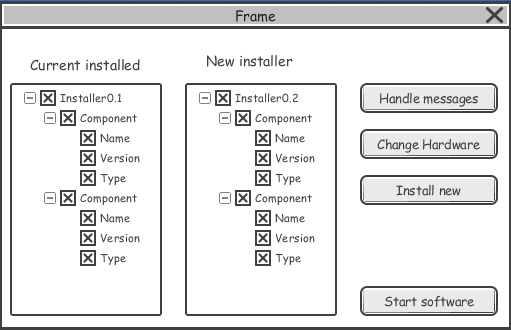
\includegraphics[scale=0.6]{afbeelding/overviewClient.png}}
\caption{Grafische user interface van de client}
\label{fig:overviewClient}

\makebox[0pt]{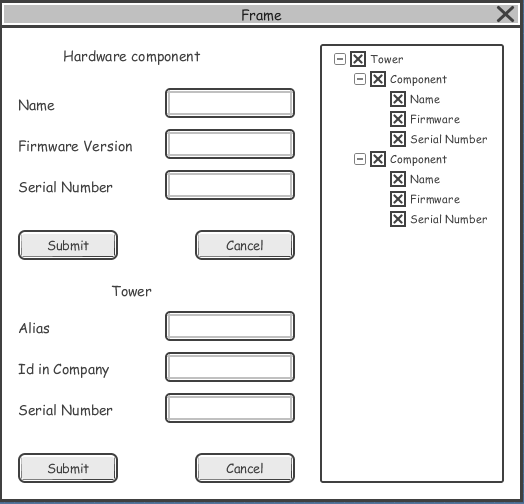
\includegraphics[scale=0.5]{afbeelding/startClient.png}}
\caption{Grafische user interface bij eerste gebruik}
\label{fig:startClient}

\end{figure}

Alle componenten samen vormen het geheel die zichtbaar was in Figuur~\vref{fig:architectuur}.
Met deze architectuur vormt een goede basis van de implementatie die in het volgende hoofdstuk besproken wordt.

